\documentclass[a4paper, 11pt, oneside]{article}

\usepackage[utf8]{inputenc}
\usepackage[T1]{fontenc}
\usepackage[french]{babel}
\usepackage{array}
\usepackage{shortvrb}
\usepackage{listings}
\usepackage[fleqn]{amsmath}
\usepackage{amsfonts}
\usepackage{fullpage}
\usepackage{enumerate}
\usepackage{graphicx}             % import, scale, and rotate graphics
\usepackage{subfigure}            % group figures
\usepackage{alltt}
\usepackage{url}
\usepackage{indentfirst}
\usepackage{eurosym}
\usepackage{listings}
\usepackage{color}
\usepackage[table,xcdraw,dvipsnames]{xcolor}

% Change le nom par défaut des listing
\renewcommand{\lstlistingname}{Extrait de Code}

% Change la police des titres pour convenir à votre seul lecteur
\usepackage{sectsty}
\allsectionsfont{\sffamily\mdseries\upshape} 
% Idem pour la table des matière.
\usepackage[nottoc,notlof,notlot]{tocbibind} 
\usepackage[titles,subfigure]{tocloft} 
\renewcommand{\cftsecfont}{\rmfamily\mdseries\upshape}
\renewcommand{\cftsecpagefont}{\rmfamily\mdseries\upshape} 

\definecolor{mygray}{rgb}{0.5,0.5,0.5}
\newcommand{\coms}[1]{\textcolor{MidnightBlue}{#1}}

\lstset{
    language=C, % Utilisation du langage C
    commentstyle={\color{MidnightBlue}}, % Couleur des commentaires
    frame=single, % Entoure le code d'un joli cadre
    rulecolor=\color{black}, % Couleur de la ligne qui forme le cadre
    stringstyle=\color{RawSienna}, % Couleur des chaines de caractères
    numbers=left, % Ajoute une numérotation des lignes à gauche
    numbersep=5pt, % Distance entre les numérots de lignes et le code
    numberstyle=\tiny\color{mygray}, % Couleur des numéros de lignes
    basicstyle=\tt\footnotesize, 
    tabsize=3, % Largeur des tabulations par défaut
    keywordstyle=\tt\bf\footnotesize\color{Sepia}, % Style des mots-clés
    extendedchars=true, 
    captionpos=b, % sets the caption-position to bottom
    texcl=true, % Commentaires sur une ligne interprétés en Latex
    showstringspaces=false, % Ne montre pas les espace dans les chaines de caractères
    escapeinside={(>}{<)}, % Permet de mettre du latex entre des <( et )>.
    inputencoding=utf8,
    literate=
  {á}{{\'a}}1 {é}{{\'e}}1 {í}{{\'i}}1 {ó}{{\'o}}1 {ú}{{\'u}}1
  {Á}{{\'A}}1 {É}{{\'E}}1 {Í}{{\'I}}1 {Ó}{{\'O}}1 {Ú}{{\'U}}1
  {à}{{\`a}}1 {è}{{\`e}}1 {ì}{{\`i}}1 {ò}{{\`o}}1 {ù}{{\`u}}1
  {À}{{\`A}}1 {È}{{\`E}}1 {Ì}{{\`I}}1 {Ò}{{\`O}}1 {Ù}{{\`U}}1
  {ä}{{\"a}}1 {ë}{{\"e}}1 {ï}{{\"i}}1 {ö}{{\"o}}1 {ü}{{\"u}}1
  {Ä}{{\"A}}1 {Ë}{{\"E}}1 {Ï}{{\"I}}1 {Ö}{{\"O}}1 {Ü}{{\"U}}1
  {â}{{\^a}}1 {ê}{{\^e}}1 {î}{{\^i}}1 {ô}{{\^o}}1 {û}{{\^u}}1
  {Â}{{\^A}}1 {Ê}{{\^E}}1 {Î}{{\^I}}1 {Ô}{{\^O}}1 {Û}{{\^U}}1
  {œ}{{\oe}}1 {Œ}{{\OE}}1 {æ}{{\ae}}1 {Æ}{{\AE}}1 {ß}{{\ss}}1
  {ű}{{\H{u}}}1 {Ű}{{\H{U}}}1 {ő}{{\H{o}}}1 {Ő}{{\H{O}}}1
  {ç}{{\c c}}1 {Ç}{{\c C}}1 {ø}{{\o}}1 {å}{{\r a}}1 {Å}{{\r A}}1
  {€}{{\euro}}1 {£}{{\pounds}}1 {«}{{\guillemotleft}}1
  {»}{{\guillemotright}}1 {ñ}{{\~n}}1 {Ñ}{{\~N}}1 {¿}{{?`}}1
}
\newcommand{\tablemat}{~}

%%%%%%%%%%%%%%%%% TITRE %%%%%%%%%%%%%%%%
\newcommand{\GrNbr}{s180498-s170220}
\newcommand{\PrenomUN}{Martin}
\newcommand{\NomUN}{RANDAXHE}
\newcommand{\PrenomDEUX}{Cyril}
\newcommand{\NomDEUX}{RUSSE}
\renewcommand{\tablemat}{\tableofcontents}

\title{\textbf{MATH0499 - Projet}\\Graphe k-dégénéré}
\author{Groupe \GrNbr : \PrenomUN~\textsc{\NomUN}, \PrenomDEUX~\textsc{\NomDEUX}}
\date{}
\begin{document}
\maketitle
\newpage
\tablemat
\newpage

%%%%%%%%%%%%%%%%%%%%%%%%%%%%%%%%%%%%%%%%%%%%%%%%
\section{\textbf{Introduction}}
Ce projet consiste en la création de deux algorithmes sur le sujet de la k-dégénérescence de graphes.
\\Le premier permet tout simplement de savoir si un graphe est k-dégénéré et de fournir, 
dans le cas positif, une suite de noeud à supprimer le prouvant.
\\En second algorithme, une implémentation créant un graphe dit de k-dégénéré maximal.


\section{\textbf{Algorithmes importants}}

\subsection{Est-k-dégénéré}

Comme introduit dans la section précédénte, cet algorithme va permettre de définir si 
le graphe, donné par l'utilisateur du programme, est ou non k-dégénéré.
\\Notre algorithme va d'abords créer une copie de la liste des noeuds du graphe. Ensuite,
nous les parcourons et vérifions leur degré si celui-ci est inférieur ou égal à la 
valeur de k, alors celui-ci est supprimé et enregistré à la suite d'une liste qui 
répertorie tous ces noeuds afin de pouvoir les enregistrer par après si le graphe 
est k-dégéré. Si en ayant parcouru tous les noeuds restants, aucun n'est de degré 
correspondant aux attentes, l'algorithme s'arrête et informe l'utilisateur que le 
graphe n'est pas k-dégénéré.
Si au contraire, il a été possible de supprimer tous les noeuds, le graphe est k-dégénéré 
et la liste de suite de noeud est écrite dans un fichier.

\subsection{Génération de graphes k-dégénérés maximaux}

Après réflexion sur les graphe k-dégénérés, nous en avons conclut que nous pouvions déjà 
répertorié 2 cas différents. Il se différencie en fonction de sa valeur de dégénérescence k 
et son nombre de noeud n. En effet, si le nombre de noeud est inférieur ou égal à 
k+1, alors tous les noeuds doivent être relié entre eux. Dès que l'on passe se cap, 
après analyse à la manière d'une démonstration par récurence, nous avons remarqué 
que les graphes maximaux respecte un paterne tel que si l'on rajoute un noeud, il 
suffit de le lier au k éléments précédents.
\\L'algorithme crée donc les noeuds 1 par 1, et pour chacun d'eux, lie directement celui-ci 
respectant les deux cas énoncés ci-dessus. Il sera finalement enregistré 
dans un fichier.


\section{\textbf{Difficultés}}

Nous allons parcourir dans cette section les points critiques des implémentations 
de ce projet et de la recherche pour celles-ci.

\subsection{Performance algorithme k-dégénéré}

De grands dilemmes nous ont étés posés pour cet algorithme. Premièrement, nous n'avons 
pas eu de meilleurs idées afin d'obtenir une meilleur complexité que $n^2$ en pire cas. 
La grande question par après a été de nous demander quels sont les cas les plus probables 
afin d'au moins obtenir un meilleur cas moyen. Le fait est que les différents cas que nous 
avons répertorié ne sont pas improbables. En effet, par exemple, avec notre implémentation 
actuelle un graphe ayant beaucoup de noeuds de degré en même temps déjà inférieur se serait 
vu plus éfficace avec un implémentation parcourant pratiquement toute la liste à chaque 
boucle afin de retirer plusieurs noeuds directement. D'autre part, cette manière aurait 
en revanche rendu les cas de graphes fort dense et se rapprochant de graphe k-dégénéré maximaux, 
nécessitant quant à eux de supprimer plus régulièrement certains noeuds avant de pouvoir 
en supprimer d'autres juste après, extrêmement moins efficace. Il était donc difficile de 
trouver une technique étant convenable quelque soit le cas. Celle que nous avons 
adoptée ne l'est en effet pas pour tous les cas.

\subsection{Cas générique pour graphes k-dégénérés maximaux}

Comme nous l'avons énoncé dans la section 2.2, afin de trouver une solution 
algorithmique à ce problème, il nous a été nécessaire de définir quels étaient 
les différents cas que nous pouvions rencontrer. Nous avons donc suivi une logique 
de démonstrations par récurence et nous avons réalisé que pour quelque soit la valeur 
de dégénérescence, les graphes ou sous-graphes des k+1 premiers éléments devait être 
tous reliés entre eux. Ensuite, pour les noeuds suivants, chaque nouveau devra 
de leur côté être reliés aux k éléments précédents. A partir du moment, où nous avons 
bel et bien vérifier que cette logique permet de couvrir tous les cas de k et de n, 
l'implémentation n'a pas été la partie la plus complexe. Et la complexité de 
l'algorithme est linéaire suivant le nombre de noeud et des arcs nécessaires. 

\section{\textbf{Utilisation des programmes}}
Nous sommes partis sur une implémentation en python en utilisant la 
bibliothèque "Networkx" conseillé dans l'énoncé. Nous avons choisi que les graphes 
qui seront donnés et que renverront les programmes suivrait un modèle de fichier 
"adjlist". Ce système de fichier répertorie tous les noeuds et pour chaque noeud 
les autres noeuds auquels il est lié. Comme son nom l'indique, telles les listes 
d'adjacences. Ceux-ci sont écrit dans des fichiers au format "txt".
\\Nous avons préféré séparé les 2 grands problèmes en 2 programmes distincts 
"k-degenere.py" et "k-degenere\_max.py". Le premier permettant de définir si un graphe 
donné en argument à l'exécution est k-dégénéré ou non et le second pour la création 
de graphe k-dégénéré maximaux.
Nous avons également fourni un troisième programme que nous aurions pu intégré dans les 2 
autres car il consiste juste à afficher graphiquement un graphe dans un fichier txt à la structure 
adjlist. Nous avions un léger quand à l'exécution de ceux-ci sur un autre ordinateur 
que l'autre vu qu'elle nécessite l'installation de la bibliothèque "matplotlib".

\subsection{k-degenere.py}

Le programme s'exécute avec python3 et nécessite l'ajout d'argument à l'exécution.
Nous allons voir en revue les options de ce programme :
\begin{itemize}
    \item -i Nom du fichier contenant le graphe
    \item -k Une valeur entière correspondant à la valeur de dégénérescence voulant être vérifiée
    \item -o (optionnel) Le nom du fichier dans lequel noté la suite de noeud dans le cas où 
    le graphe est k-dégénéré. Cette option est optionnel. Si elle n'est pas donnée 
    le programme écrira par défaut dans un fichier "default.txt".
    \item -h (optionnel) Cette option ne nécessite pas d'argument et permet juste d'afficher l'aide.
\end{itemize}

Voici quelques exemples d'exécutions :
\begin{figure}[h]
    \centering
    \includegraphics[scale=0.38]{exécutions_k_degenere.png}
    \caption{Exemples d'exécutions de k-degenere.py}
\end{figure}

\newpage
\subsection{k-degenere\_max.py}

Ce programme s'exécute de la même manière que pour k-degenere.py, mais leurs 
options diffèrent. Ce programme ci va produire un graphe k-degenere maximal avec 
n noeud. K et n sont des paramètres à transmettre à l'exécution et un nom 
de fichier dans lequel enregistrer le graphe au format txt suivant la structure 
"adjlist" peut être donné.

\begin{itemize}
    \item -k Une valeur entière correspondante à la valeur de dégénérescence voulue.
    \item -n Une valeur entière correspondante aux nombres de noeuds désiré.
    \item -o (optionnel) Le nom du fichier dans lequel enregister le graphe nouvellement créé. 
    Par défaut, le nom de fichier sera "k-degenere\_max.txt".
    \item -h (optionnel) Cette option ne nécessite pas d'argument et permet juste d'afficher l'aide.
\end{itemize}

Voici quelques exemples d'exécutions :
\begin{figure}[h]
    \centering
    \includegraphics[scale=0.38]{exécutions_k_degenere_max.png}
    \caption{Exemples d'exécutions de k-degenere\_max.py}
\end{figure}

\subsection{affichage\_graphe.py}
Ce programme nécessite l'installation de la bibliothèque matplotlib.
Ce programme permet d'afficher les graphes écrit sous forme d'"adjlist" dans des 
fichiers txt.

Il nécessite uniquement l'option -i suivi du nom du fichier contenant le 
graphe à afficher.

Voici un exemple d'affichage du programme avec l'utilisation du graphe contenu dans 
le fichier d'exemple "graphe\_test.txt".

\begin{figure}[h]
    \centering
    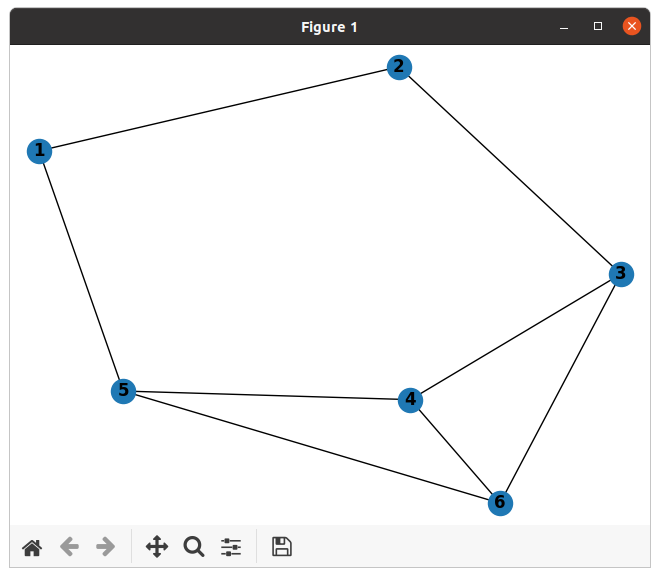
\includegraphics[scale=0.38]{affichage_graphe.png}
    \caption{Exemples d'affichage graphique d'un graphe}
\end{figure}










\end{document}
